\documentclass[./PianodiProgetto.tex]{subfiles}

\begin{document}
	
\chapter{Preventivo}
I periodi di Analisi e di Consolidamento dei requisiti sono considerati di investimento e quindi non a carico del committente. Le ore relative qui rendicontate non saranno conteggiate nelle ore totali da retribuire.\\
La suddivisione oraria viene fatta tenendo conto di tre regole principali:
\begin{enumerate}
\item Ogni membro del gruppo dovrà sostenere una quantità di lavoro paragonabile, quindi il totale delle ore dovrà essere equamente distribuito tra i membri;
\item Ogni membro del gruppo dovrà ricoprire ogni ruolo almeno una volta;
\item In nessun caso si dovrà verificare un conflitto di interessi in cui un \textit{Vericatore} debba controllare il proprio lavoro.
\end{enumerate}
Le sigle utilizzate per i vari ruoli saranno:
\begin{itemize}
\item Re: \textit{Responsabile};
\item Am: \textit{Amministratore};
\item An: \textit{Analista};
\item Pt: \textit{Progettista};
\item Pr: \textit{Programmatore};
\item Ve: \textit{Verificatore}.
\end{itemize}
\noindent Ogni sezione rappresenta un periodo di lavoro del progetto ed è suddivisa in prospetto orario dove si espone la distribuzione oraria di ogni componente del gruppo nei vari ruoli che ricopre e in prospetto economico dove si riassumono i costi sostenuti per ogni ruolo. \\
Ogni prospetto è accompagnato da un grafico che permette una veloce comprensione della suddivisione delle ore nei vari ruoli. Per il prospetto orario si utilizza un diagramma a barre mentre per quello economico un diagramma a torta.\\
\noindent Per facilitare la lettura delle tabelle si è deciso che, nel caso una cella contenga un valore pari a 0, questo verrà omesso lasciando la cella vuota.

\section{Analisi}
Questo periodo di lavoro fa parte del periodo di investimento a carico del gruppo Graphite.
\subsection{Prospetto Orario}
Nel periodo di Analisi la distribuzione oraria sarà la seguente:

\begin{table}[H]
	\centering
	\begin{tabular}{|c|cccccc|c|}
		\hline
		Nominativo&Re&Am&An&Pt&Pr&Ve&Ore totali\\ \hline
		Marco Focchiatti&5& &16& & & &21 \\ \hline
		Samuele Modena&10&4& & & &8&22 \\ \hline
		Matteo Rizzo&9& & & & &12&21 \\ \hline
		Giulio Rossetti& &8&6& & &8&22 \\ \hline
		Kevin Silvestri& & &11& & &10&21 \\ \hline
		Manfredi Smaniotto& & &14& & &8&22 \\ \hline
		Cristiano Tessarolo& &8&14& & & &22 \\  \hline
		Ore totali ruolo&24&20&61& & &46&151 \\ \hline
	\end{tabular}
\caption{Distribuzione oraria del periodo di Analisi}
\end{table}

Tali dati sono riassunti graficamente nel seguente diagramma a barre:
\begin{figure}[H]
	\centering
	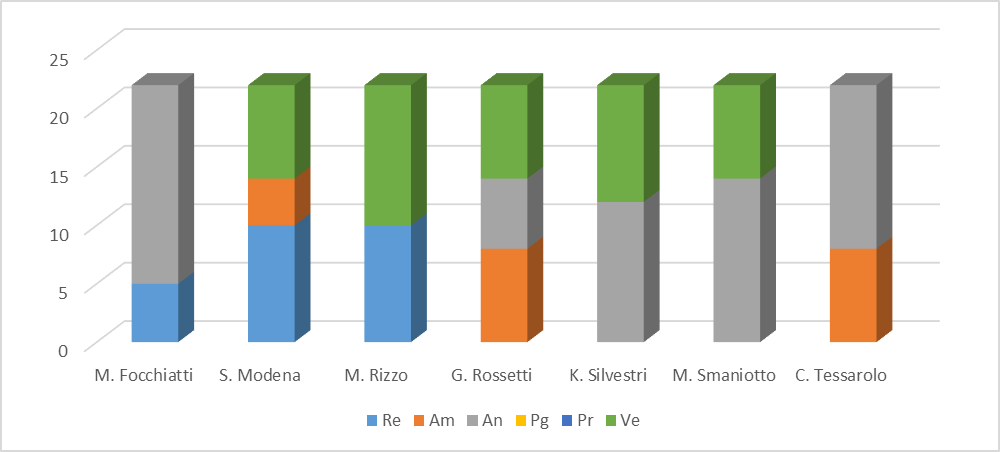
\includegraphics[width=1\linewidth]{img/grafici/AnalisiProspettoOrario}
	\caption{Grafico suddivisione oraria del periodo di Analisi}
	\label{fig:analisi-prospetto-orario}
\end{figure}

\subsection{Prospetto Economico}
Nello svolgimento delle attività di questo periodo i costi sostenuti per ogni ruolo, non a carico del proponente trattandosi dell’investimento iniziale, sono riassunti nella seguente tabella:

\begin{table}[H]
	\centering
	\begin{tabular}{|c|c|c|}
		\hline
		Ruolo&Ore&Costo in \euro{} \\ \hline
		Responsabile&24&720,00  \\ \hline
		Amministratore&20&400,00  \\ \hline
		Analista&61&1525,00  \\ \hline
		Progettista& &  \\ \hline
		Programmatore& &  \\ \hline
		Verificatore&46&690,00  \\ \hline
		Totale&151&3335,00 \\ \hline
	\end{tabular}
	\caption{Prospetto economico del periodo di Analisi}
\end{table}

La ripartizione delle ore tra i vari ruoli è rappresentata graficamente tramite il seguente diagramma a torta:

\begin{figure}[H]
	\centering
	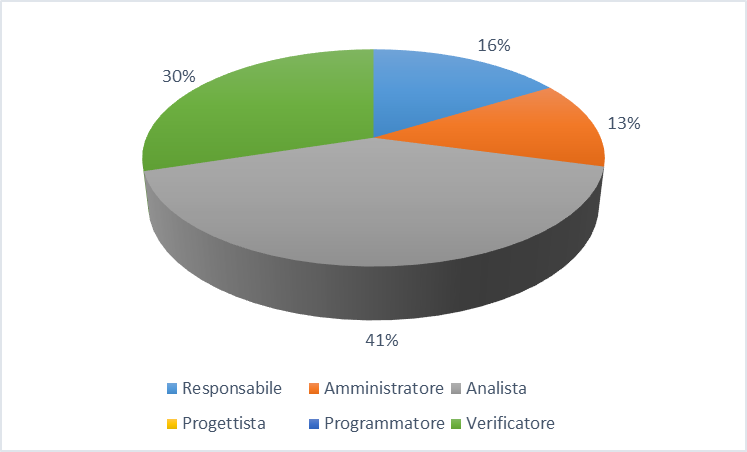
\includegraphics[width=1\linewidth]{img/grafici/AnalisiProspettoEconomico}
	\caption{Grafico suddivisione dei ruoli del periodo di Analisi}
	\label{fig:analisi-prospetto-economico}
\end{figure}


\section{Consolidamento dei requisiti}
Questo periodo di lavoro fa parte del periodo di investimento a carico del gruppo Graphite.
\subsection{Prospetto Orario}
Nel periodo di Consolidamento dei requisiti la distribuzione oraria sarà la seguente:

\begin{table}[H]
	\centering
	\begin{tabular}{|c|cccccc|c|}
		\hline
		Nominativo&Re&Am&An&Pt&Pr&Ve&Ore totali\\ \hline
		Marco Focchiatti&3& &5& & & &8 \\ \hline
		Samuele Modena& & &7& & & &7 \\ \hline
		Matteo Rizzo& & &2&4& & &6 \\ \hline
		Giulio Rossetti&2& & & & &4&6 \\ \hline
		Kevin Silvestri& &6& & & & &6 \\ \hline
		Manfredi Smaniotto& & &3& & &4&7 \\ \hline
		Cristiano Tessarolo& & & & & &7&7 \\  \hline
		Ore totali ruolo&5&8&19& & &15&47 \\ \hline
	\end{tabular}
	\caption{Distribuzione oraria del periodo di Consolidamento dei requisiti}
\end{table}

Tali dati sono riassunti graficamente nel seguente diagramma a barre:
\begin{figure}[H]
	\centering
	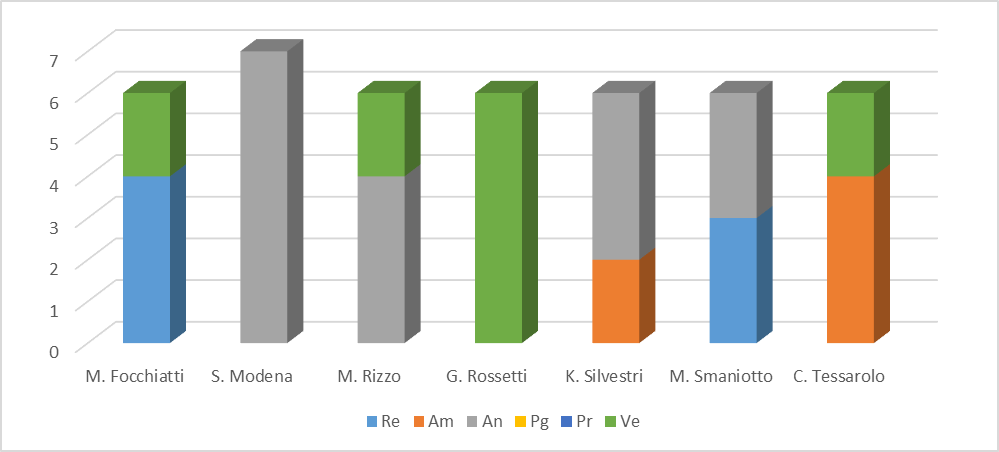
\includegraphics[width=1\linewidth]{img/grafici/ConsolidamentoRequisitiProspettoOrario}
	\caption{Grafico suddivisione oraria del periodo di Consolidamento dei requisiti}
	\label{fig:consolidamento-requisiti-prospetto-orario}
\end{figure}

\subsection{Prospetto Economico}
Nello svolgimento delle attività di questo periodo i costi sostenuti per ogni ruolo sono riassunti nella seguente tabella:

\begin{table}[H]
	\centering
	\begin{tabular}{|c|c|c|}
		\hline
		Ruolo&Ore&Costo in \euro{} \\ \hline
		Responsabile&5&150,00  \\ \hline
		Amministratore&8&160,00  \\ \hline
		Analista&19&475,00  \\ \hline
		Progettista& &  \\ \hline
		Programmatore& &  \\ \hline
		Verificatore&15&225,00  \\ \hline
		Totale&47&1010,00 \\ \hline
	\end{tabular}
	\caption{Prospetto economico del periodo di Consolidamento dei requisiti}
\end{table}

La ripartizione delle ore tra i vari ruoli è rappresentata graficamente tramite il seguente diagramma a torta:
\begin{figure}[H]
	\centering
	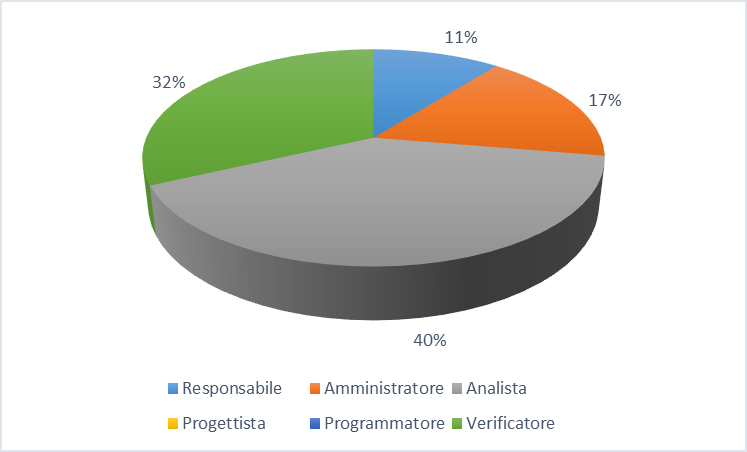
\includegraphics[width=1\linewidth]{img/grafici/ConsolidamentoRequisitiProspettoEconomico}
	\caption{Grafico suddivisione dei ruoli del periodo di Consolidamento dei requisiti}
	\label{fig:consolidamento-requisiti-prospetto-economico}
\end{figure}

\section{Progettazione architetturale}
Questo periodo di lavoro fa parte del periodo del preventivo.
\subsection{Prospetto Orario}
Nel periodo di Progettazione architetturale la distribuzione oraria sarà la seguente:

\begin{table}[H]
	\centering
	\begin{tabular}{|c|cccccc|c|}
		\hline
		Nominativo&Re&Am&An&Pt&Pr&Ve&Ore totali\\ \hline
		Marco Focchiatti&2&5& & & &23&30 \\ \hline
		Samuele Modena& & &12&18& & &30 \\ \hline
		Matteo Rizzo& & &8&22& & &30 \\ \hline
		Giulio Rossetti& & & &15& &15&30 \\ \hline
		Kevin Silvestri&8& & & & &22&30 \\ \hline
		Manfredi Smaniotto& &5& &25& & &30 \\ \hline
		Cristiano Tessarolo& & & &30& & &30 \\  \hline
		Ore totali ruolo&10&10&20&110& &60&210 \\ \hline
	\end{tabular}
	\caption{Distribuzione oraria del periodo di Progettazione architetturale}
\end{table}

Tali dati sono riassunti graficamente nel seguente diagramma a barre:
\begin{figure}[H]
	\centering
	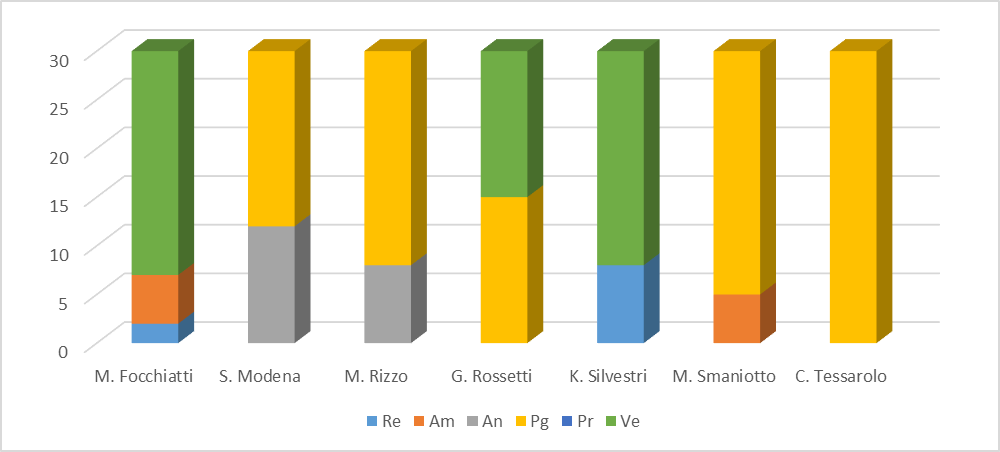
\includegraphics[width=1\linewidth]{img/grafici/ProgettazioneArchitetturaleProspettoOrario}
	\caption{Grafico suddivisione oraria del periodo di Progettazione architetturale}
	\label{fig:progettazione-architetturale-prospetto-orario}
\end{figure}

\subsection{Prospetto Economico}
Nello svolgimento delle attività di questo periodo i costi sostenuti per ogni ruolo sono riassunti nella seguente tabella:

\begin{table}[H]
	\centering
	\begin{tabular}{|c|c|c|}
		\hline
		Ruolo&Ore&Costo in \euro{} \\ \hline
		Responsabile&10&300,00  \\ \hline
		Amministratore&10&200,00  \\ \hline
		Analista&20&500,00  \\ \hline
		Progettista&110&2420,00  \\ \hline
		Programmatore& &  \\ \hline
		Verificatore&60&900,00  \\ \hline
		Totale&210&4320,00 \\ \hline
	\end{tabular}
	\caption{Prospetto economico del periodo di Progettazione architetturale}
\end{table}

La ripartizione delle ore tra i vari ruoli è rappresentata graficamente tramite il seguente diagramma a torta:
\begin{figure}[H]
	\centering
	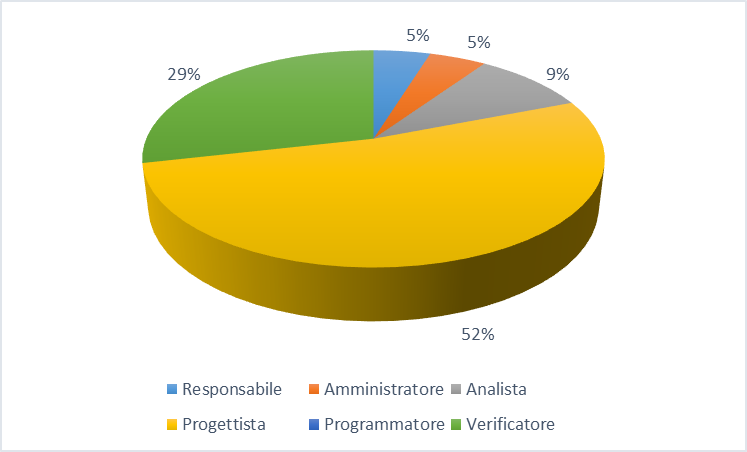
\includegraphics[width=1\linewidth]{img/grafici/ProgettazioneArchitetturaleProspettoEconomico}
	\caption{Grafico suddivisione dei ruoli del periodo di Progettazione architetturale}
	\label{fig:progettazione-architetturale-prospetto-economico}
\end{figure}

\section{Progettazione di dettaglio e codifica}
Questo periodo di lavoro fa parte del periodo del preventivo.
\subsection{Prospetto Orario}
Nel periodo di Progettazione di dettaglio e codifica la distribuzione oraria sarà la seguente:

\begin{table}[H]
	\centering
	\begin{tabular}{|c|cccccc|c|}
		\hline
		Nominativo&Re&Am&An&Pt&Pr&Ve&Ore totali\\ \hline
		Marco Focchiatti& & & &30&22& &52 \\ \hline
		Samuele Modena& & & &16&10&26&52 \\ \hline
		Matteo Rizzo& &8& &14&22&8&52 \\ \hline
		Giulio Rossetti& & &5&19&22&6&52 \\ \hline
		Kevin Silvestri& & & &35&17& &52 \\ \hline
		Manfredi Smaniotto&6& & &5&17&24&52 \\ \hline
		Cristiano Tessarolo&8& & & &21&23&52 \\  \hline
		Ore totali ruolo&14&8&5&119&131&87&364 \\ \hline
	\end{tabular}
	\caption{Distribuzione oraria del periodo di Progettazione di dettaglio e codifica}
\end{table}

Tali dati sono riassunti graficamente nel seguente diagramma a barre:
\begin{figure}[H]
	\centering
	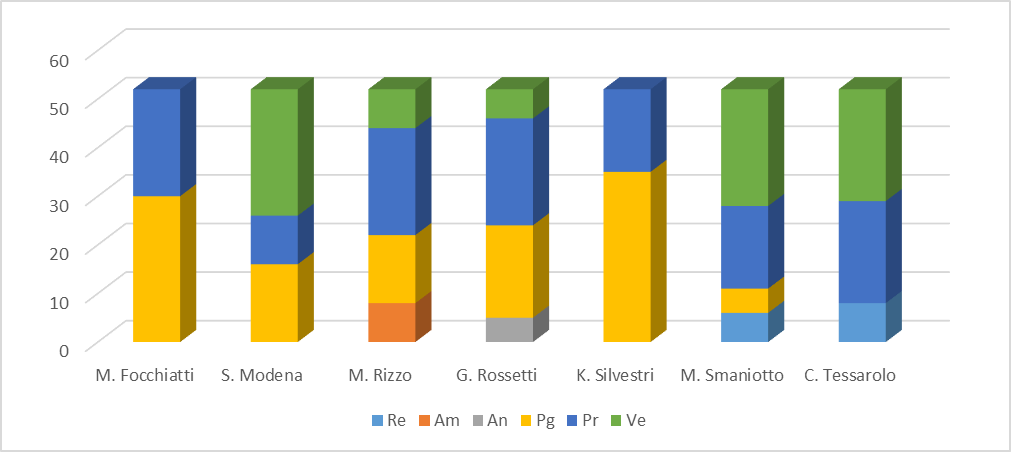
\includegraphics[width=1\linewidth]{img/grafici/ProgettazioneDettaglioCodificaProspettoOrario}
	\caption{Grafico suddivisione oraria del periodo di Progettazione di dettaglio e codifica}
	\label{fig:progettazione-dettaglio-codifica-prospetto-orario}
\end{figure}

\subsection{Prospetto Economico}
Nello svolgimento delle attività di questo periodo i costi sostenuti per ogni ruolo sono riassunti nella seguente tabella:

\begin{table}[H]
	\centering
	\begin{tabular}{|c|c|c|}
		\hline
		Ruolo&Ore&Costo in \euro{} \\ \hline
		Responsabile&14&420,00  \\ \hline
		Amministratore&8&160,00  \\ \hline
		Analista&5&125,00 \\ \hline
		Progettista&119&2618,00  \\ \hline
		Programmatore&131&1965,00  \\ \hline
		Verificatore&87&1305,00  \\ \hline
		Totale&364&6593,00 \\ \hline
	\end{tabular}
	\caption{Prospetto economico del periodo di Progettazione di dettaglio e codifica}
\end{table}

La ripartizione delle ore tra i vari ruoli è rappresentata graficamente tramite il seguente diagramma a torta:

\begin{figure}[H]
	\centering
	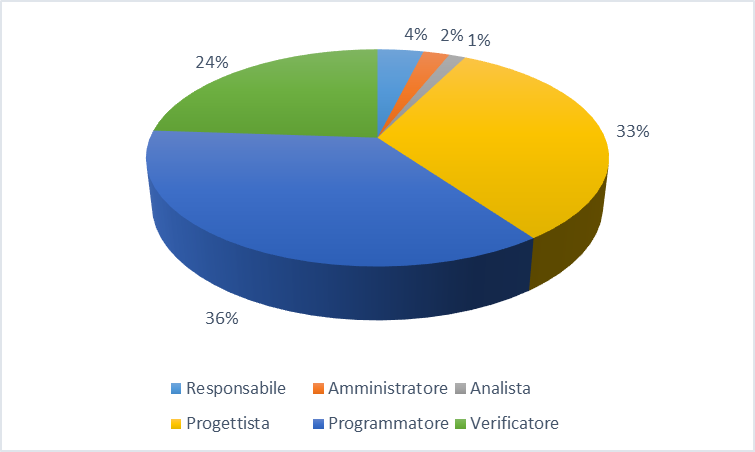
\includegraphics[width=1\linewidth]{img/grafici/ProgettazioneDettaglioCodificaProspettoEconomico}
	\caption{Grafico suddivisione dei ruoli del periodo di Progettazione di dettaglio e codifica}
	\label{fig:progettazione-dettaglio-codifica-prospetto-economico}
\end{figure}

\section{Validazione e collaudo}
Questo periodo di lavoro fa parte del periodo del preventivo.
\subsection{Prospetto Orario}
Nel periodo di Validazione e collaudo la distribuzione oraria sarà la seguente:

\begin{table}[H]
	\centering
	\begin{tabular}{|c|cccccc|c|}
		\hline
		Nominativo&Re&Am&An&Pt&Pr&Ve&Ore totali\\ \hline
		Marco Focchiatti& & & &2& &18&20 \\ \hline
		Samuele Modena& &6& & &14& &20 \\ \hline
		Matteo Rizzo& &2& &6& &12&20 \\ \hline
		Giulio Rossetti&10& & &6& &4&20 \\ \hline
		Kevin Silvestri& &2& & &5&13&20 \\ \hline
		Manfredi Smaniotto&2&4& &4&4&6&20 \\ \hline
		Cristiano Tessarolo& & & &4& &16&20 \\  \hline
		Ore totali ruolo&12&14& &22&23&69&140 \\ \hline
	\end{tabular}
	\caption{Distribuzione oraria del periodo di Validazione e collaudo}
\end{table}

Tali dati sono riassunti graficamente nel seguente diagramma a barre:
\begin{figure}[H]
	\centering
	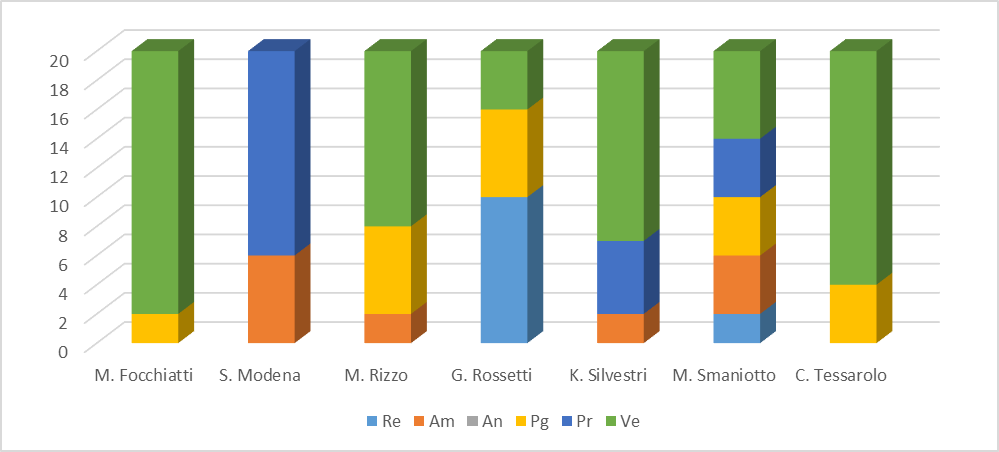
\includegraphics[width=1\linewidth]{img/grafici/ValidazioneCollaudoProspettoOrario}
	\caption{Grafico suddivisione oraria del periodo di Validazione e collaudo}
	\label{fig:validazione-collaudo-prospetto-orario}
\end{figure}

\subsection{Prospetto Economico}
Nello svolgimento delle attività di questo periodo i costi sostenuti per ogni ruolo, non a carico del proponente trattandosi dell’investimento iniziale, sono riassunti nella seguente tabella:

\begin{table}[H]
	\centering
	\begin{tabular}{|c|c|c|}
		\hline
		Ruolo&Ore&Costo in \euro{} \\ \hline
		Responsabile&12&360,00  \\ \hline
		Amministratore&14&280,00  \\ \hline
		Analista& &  \\ \hline
		Progettista&22&484,00  \\ \hline
		Programmatore&23&345,00  \\ \hline
		Verificatore&69&1035,00  \\ \hline
		Totale&140&2504,00 \\ \hline
	\end{tabular}
	\caption{Prospetto economico del periodo di Validazione e collaudo}
\end{table}

La ripartizione delle ore tra i vari ruoli è rappresentata graficamente tramite il seguente diagramma a torta:

\begin{figure}[H]
	\centering
	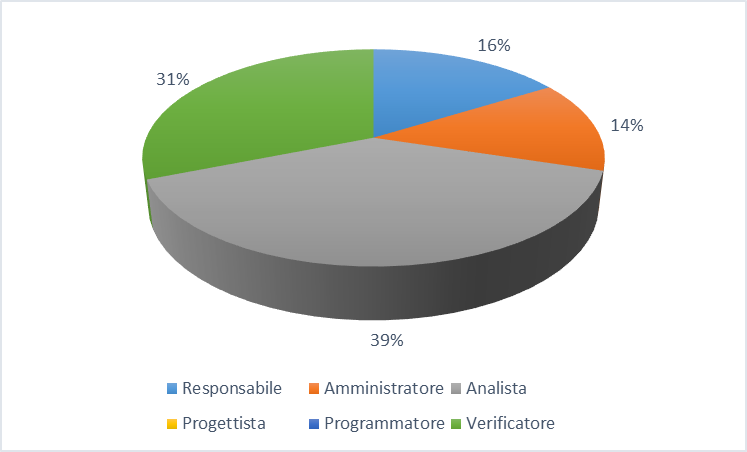
\includegraphics[width=1\linewidth]{img/grafici/ValidazioneCollaudoProspettoEconomico}
	\caption{Grafico suddivisione dei ruoli del periodo di Validazione e collaudo}
	\label{fig:validazione-collaudo-prospetto-economico}
\end{figure}

\section{Totale}
\subsection{Totale suddivisione ore con investimento}
Di seguito sono riportate il totale delle ore del progetto contando le ore di investimento e delle ore rendicontate nel preventivo a carico del committente:

\begin{table}[H]
	\centering
	\begin{tabular}{|c|cccccc|c|}
		\hline
		Nominativo&Re&Am&An&Pt&Pr&Ve&Ore totali\\ \hline
		Marco Focchiatti&10&5&21&32&22&41&131 \\ \hline
		Samuele Modena&10&10&19&34&24&34&131 \\ \hline
		Matteo Rizzo&9&12&12&42&22&32&129 \\ \hline
		Giulio Rossetti&12&8&11&40&22&37&130 \\ \hline
		Kevin Silvestri&8&8&11&35&22&45&129 \\ \hline
		Manfredi Smaniotto&8&9&17&34&21&42&131 \\ \hline
		Cristiano Tessarolo&8&8&14&34&21&46&131 \\  \hline
		Ore totali ruolo&65&60&105&251&154&277&912 \\ \hline
	\end{tabular}
	\caption{Distribuzione oraria totale delle ore di investimento e rendicontate}
\end{table}

Tali dati sono riassunti graficamente nel seguente diagramma a barre:
\begin{figure}[H]
	\centering
	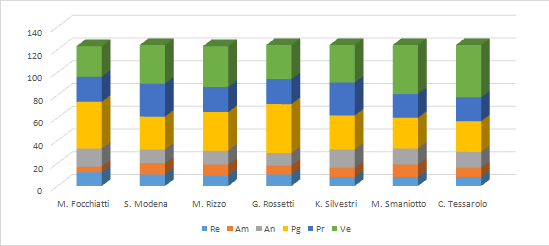
\includegraphics[width=1\linewidth]{img/grafici/OreInvestimentoRendicontateProspettoOrario}
	\caption{Grafico suddivisione oraria totale delle ore di investimento e rendicontate}
	\label{fig:ore-investimento-rendicontate-prospetto-orario}
\end{figure}

\subsection{Totale del prospetto economico con investimento}
Di seguito è riportato il totale delle ore dei diversi ruoli del progetto contando anche le ore di investimento, non a carico del proponente trattandosi dell'investimento iniziale:

\begin{table}[H]
	\centering
	\begin{tabular}{|c|c|c|}
		\hline
		Ruolo&Ore&Costo in \euro{} \\ \hline
		Responsabile&65&1950,00  \\ \hline
		Amministratore&60&1200,00  \\ \hline
		Analista&105&2625,00 \\ \hline
		Progettista&251&5522,00 \\ \hline
		Programmatore&154&2310,00 \\ \hline
		Verificatore&277&4155,00  \\ \hline
		Totale&912&17762,00 \\ \hline
	\end{tabular}
	\caption{Prospetto economico totale delle ore di investimento e rendicontate}
\end{table}

La ripartizione delle ore tra i vari ruoli è rappresentata graficamente tramite il seguente diagramma a torta:

\begin{figure}[H]
	\centering
	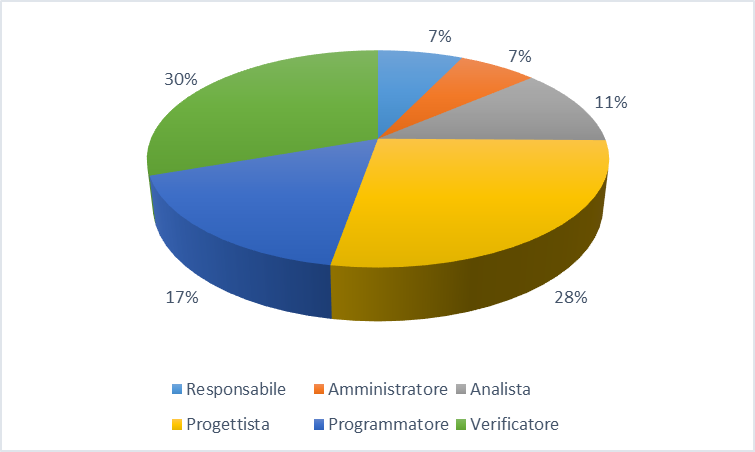
\includegraphics[width=1\linewidth]{img/grafici/OreInvestimentoRendicontateProspettoEconomico}
	\caption{Grafico suddivisione dei ruoli totale delle ore di investimento e rendicontate}
	\label{fig:ore-investimento-rendicontate-prospetto-economico}
\end{figure}


\subsection{Totale suddivisione ore rendicontate}
Di seguito sono riportate il totale delle sole ore rendicontate nel preventivo a carico del committente:

\begin{table}[H]
	\centering
	\begin{tabular}{|c|cccccc|c|}
		\hline
		Nominativo&Re&Am&An&Pt&Pr&Ve&Ore totali\\ \hline
		Marco Focchiatti&2&5& &32&22&41&102 \\ \hline
		Samuele Modena& &6&12&34&24&26&102 \\ \hline
		Matteo Rizzo& &10&8&42&22&20&102 \\ \hline
		Giulio Rossetti&10& &5&40&22&25&102 \\ \hline
		Kevin Silvestri&8&2& &35&22&35&102 \\ \hline
		Manfredi Smaniotto&8&9& &34&21&30&102 \\ \hline
		Cristiano Tessarolo&8& & &34&21&39&102 \\  \hline
		Ore totali ruolo&36&32&25&251&154&216&714 \\ \hline
	\end{tabular}
	\caption{Distribuzione oraria totale delle ore rendicontate}
\end{table}

Tali dati sono riassunti graficamente nel seguente diagramma a barre:
\begin{figure}[H]
	\centering
	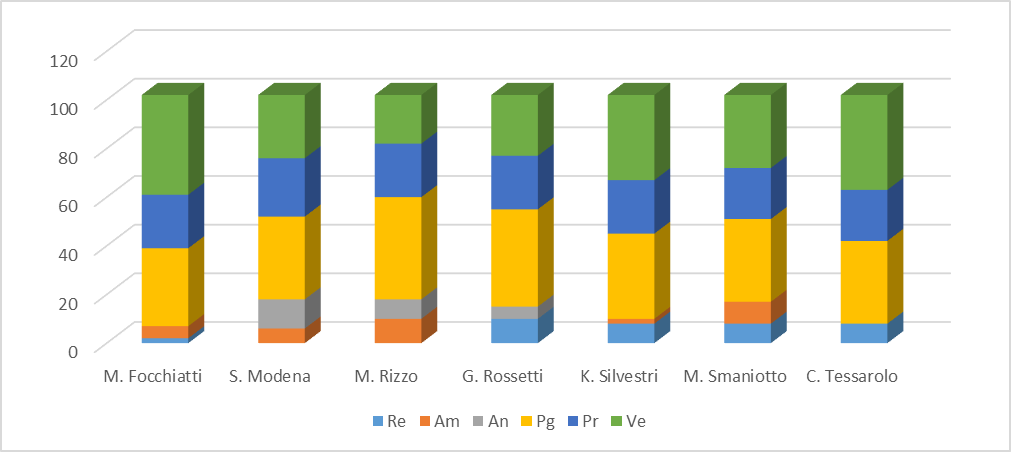
\includegraphics[width=1\linewidth]{img/grafici/OreRendicontateProspettoOrario}
	\caption{Grafico suddivisione oraria totale delle ore rendicontate}
	\label{fig:ore-rendicontate-prospetto-orario}
\end{figure}

\subsection{Totale del prospetto economico rendicontato}
Di seguito è riportato il totale delle ore dei diversi ruoli del progetto contando solo le ore rendicontate nel preventivo a carico del committente cioè dei periodi di Progettazione architetturale, Progettazione di dettaglio e codifica ed il periodo di Validazione e collaudo:

\begin{table}[H]
	\centering
	\begin{tabular}{|c|c|c|}
		\hline
		Ruolo&Ore&Costo in \euro{} \\ \hline
		Responsabile&36&1080,00 \\ \hline
		Amministratore&32&640,00 \\ \hline
		Analista&25&625,00 \\ \hline
		Progettista&251&5522,00 \\ \hline
		Programmatore&154&2310,00 \\ \hline
		Verificatore&216&3240,00 \\ \hline
		Totale&714&13417,00 \\ \hline
	\end{tabular}
	\caption{Prospetto economico totale delle ore rendicontate}
\end{table}

La ripartizione delle ore tra i vari ruoli è rappresentata graficamente tramite il seguente diagramma a torta:

\begin{figure}[H]
	\centering
	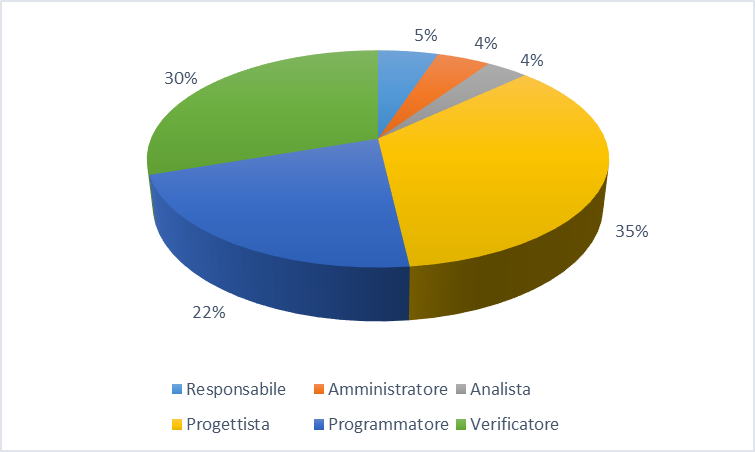
\includegraphics[width=1\linewidth]{img/grafici/OreRendicontateProspettoEconomico}
	\caption{Grafico suddivisione dei ruoli totale delle ore rendicontate}
	\label{fig:ore-rendicontate-prospetto-economico}
\end{figure}

\section{Conclusione}
Il costo totale preventivato per il progetto è di 13417,00 \euro{}.

\chapter{Consuntivo e Preventivo a finire}
In questa sezione verranno presentati i consuntivi dei vari periodi con una
breve valutazione degli stessi. Verrà inoltre presentato un preventivo a finire
che terrà conto dei soli periodi rendicontati. I valori presentati saranno:
\begin{itemize}
\item \textbf{Positivi:} se il preventivo è superiore ai valori del consuntivo;
\item \textbf{Negativi:} se il preventivo è inferiore ai valori del consuntivo.
\end{itemize}
\section{Periodo di Analisi}
Essendo il periodo di Analisi considerato periodo di investimento, il consuntivo viene presentato a scopo informativo ma non conteggiato nel preventivo a finire.
\subsection{Consuntivo}
Di seguito è presentata la tabella contenente i dati del consuntivo per il
periodo di Analisi.

\begin{table}[H]
	\centering
	\begin{tabular}{|c|c|c|c|c|}
		\hline
	 	 & \multicolumn{2}{c|}{Ore} & \multicolumn{2}{c|}{Costo in \euro{}}  \\ \hline
		Ruolo&Preventivo&Consuntivo&Preventivo&Consuntivo \\ \hline
		Responsabile&24&24&720,00&720,00  \\ \hline
		Amministratore&20&19(+1)&400,00&380,00(+20)  \\ \hline
		Analista&61&67(-6)&1525,00&1675(-150)  \\ \hline
		Progettista& & & &  \\ \hline
		Programmatore& & & &  \\ \hline
		Verificatore&46&46&690,00&690,00  \\ \hline
		Totale&151&156&3335,00&3465,00  \\ \hline
		Differenza& \multicolumn{2}{c|}{-5 Ore} & \multicolumn{2}{c|}{-130,00 \euro{}} \\ \hline
	\end{tabular}
	\caption{Prospetto orario ed economico a consuntivo del periodo di Analisi}
\end{table}

\subsection{Conclusione}
Nell'esecuzione del primo periodo di Analisi è stato necessario usare più
ore del previsto per il ruolo di Analista mentre si è riusciti a risparmiare nel ruolo di Amministratore. Questo è dovuto
probabilmente ad una sottostima del carico di lavoro presentato dalla Analisi
dei Requisiti. Le ore di verifica invece, si sono dimostrate sufficienti a svolgere
le attività previste. Il risultato del periodo è complessivamente di cinque ore
lavorative oltre il previsto, con una spesa aggiuntiva di 130,00 \euro{}.
\section{Preventivo a finire}
Viene qui presentata una tabella contenente l'attuale preventivo a finire.
Vengono inseriti i valori del periodo di Analisi e Consolidamento dei requisiti
a scopo riassuntivo, tuttavia essi non verranno conteggiati nel calcolo delle
ore rendicontate. Se il valore del consuntivo non fosse ancora presente, verrà
usato il valore del preventivo.

\begin{table}[H]
	\centering
	\begin{tabular}{|c|c|c|}
		\hline
		Periodo&Preventivo \euro{}&Consuntivo \euro{} \\ \hline
		Analisi&3415,00&3465,00  \\ \hline
		Consolidamento dei requisiti&1010,00&Non presente  \\ \hline
		\multicolumn{3}{|c|}{Rendicontato}  \\ \hline
		Progettazione architetturale&4320,00&Non presente  \\ \hline
		Progettazione di dettaglio e codifica&6593,00&Non presente  \\ \hline
		Validazione e collaudo&2504,00&Non presente  \\ \hline
		Totale&17842,00&17892,00 \\ \hline
		Rendicontato&13417,00&13417,00 \\ \hline
	\end{tabular}
	\caption{Preventivo a finire}
\end{table}

\appendix


\appendix

\chapter{Rilevazione dei rischi}

\section{Analisi}

\begin{itemize}
	\item \textbf{Codice:} RT0;
	\begin{itemize}
		\item \textbf{Descrizione:} alcuni membri del gruppo non erano pratici con Git e \LaTeX;
		\item \textbf{Contromisure:} è stato spiegato loro l'utilizzo di queste tecnologie.
	\end{itemize} 
	\item \textbf{Codice:} RG1;
	\begin{itemize}
		\item \textbf{Descrizione:} a causa delle festività invernali e/o problemi personali, alcuni membri del gruppo si sono assentati per alcuni giorni;
		\item \textbf{Contromisure:} l'eventuali assenze sono state comunicate con largo anticipo, ciò ha permesso di organizzare il lavoro in modo ottimale tenendo conto delle assenze.
	\end{itemize} 
\end{itemize}

\chapter{Organigramma}

\section{Redazione}
\begin{table}[H]
	\centering
	\begin{tabular}{|c|c|c|}
		\hline
		Nome&Data&Firma \\ \hline
		Matteo Rizzo& 12-12-2017 &
\includegraphics[scale=0.5]{img/firme/RizzoMatteo} \\
		\hline
	\end{tabular}
	\caption{Redazione}
\end{table}

\section{Approvazione}
\begin{table}[H]
	\centering
	\begin{tabular}{|c|c|c|}
		\hline
		Nome&Data&Firma \\ \hline
		Matteo Rizzo& 12-12-2017 & 
\includegraphics[scale=0.5]{img/firme/RizzoMatteo} \\
		\hline
	\end{tabular}
	\caption{Approvazione}
\end{table}

\section{Accettazione dei componenti}
\begin{table}[H]
	\centering
	\begin{tabular}{|c|c|c|}
		\hline
		Nome&Data&Firma \\ \hline
		Marco Focchiatti& 12-12-2017 &
\includegraphics[scale=0.5]{img/firme/FocchiattiMarco} \\ \hline
		Samuele Modena& 12-12-2017 &
\includegraphics[scale=0.5]{img/firme/ModenaSamuele} \\ \hline
		Matteo Rizzo& 12-12-2017 &
\includegraphics[scale=0.5]{img/firme/RizzoMatteo} \\ \hline
		Giulio Rossetti&  12-12-2017 &
\includegraphics[scale=0.5]{img/firme/RossettiGiulio} \\ \hline
		Kevin Silvestri& 12-12-2017 &
\includegraphics[scale=0.5]{img/firme/SilvestriKevin} \\ \hline
		Manfredi Smaniotto& 12-12-2017 &
\includegraphics[scale=0.5]{img/firme/SmaniottoManfredi} \\ \hline
		Cristiano Tessarolo& 12-12-2017 &
\includegraphics[scale=0.5]{img/firme/TessaroloCristiano} \\  
		\hline
	\end{tabular}
	\caption{Accettazione dei componenti}
\end{table}

\section{Componenti}
\begin{table}[H]
	\begin{tabular}{|c|c|c|}
	\hline
	Nome&Matricola&Indirizzo email \\ \hline
	Marco Focchiatti&1121294&marco.focchiatti@studenti.unipd.it  \\ \hline
	Samuele Modena&1099080&samuele.modena@studenti.unipd.it \\ \hline
	Matteo Rizzo&1123496&matteo.rizzo.4@studenti.unipd.it \\ \hline
	Giulio Rossetti&1122603&giulio.rossetti@studenti.unipd.it \\ \hline
	Kevin Silvestri&1094138&kevin.silvestri@studenti.unipd.it \\ \hline
	Manfredi Smaniotto&1123057&manfredi.smaniotto@studenti.unipd.it \\ \hline
	Cristiano Tessarolo&1119924&cristiano.tessarolo@studenti.unipd.it \\  
	\hline
	\end{tabular}
\caption{Elenco dei componenti}
\end{table}

\section{Definizione dei ruoli}
I membri del gruppo, durante lo svolgimento del progetto, andranno a ricoprire diversi ruoli. Questi ultimi rappresentano figure aziendali specializzate, alle quali corrisponde un costo orario espresso in euro. \\
Durante tutta la durata del progetto ogni componente del gruppo dovrà ricoprire almeno una volta ogni ruolo. Al fine di evitare il conflitto di interesse va certificato che non vi siano intervalli di tempo in cui una risorsa sia anche verificatrice di se stessa.


\end{document}